\documentclass[9pt,twocolumn,twoside]{osajnl}
%% Please use 11pt if submitting to AOP
% \documentclass[11pt,twocolumn,twoside]{osajnl}

\usepackage{algorithm,algpseudocode,float}
\usepackage{lipsum}
\usepackage{graphicx}
\usepackage{subfigure}
\usepackage{natbib}
\setcitestyle{square}

\renewcommand{\bibname}{reference}
\newcommand{\HR}{\rule{1em}{0.4pt}}
\renewcommand{\algorithmicrequire}{\textbf{Input:}} %Use Input in the format of Algorithm
\renewcommand{\algorithmicensure}{\textbf{Output:}} %UseOutput in the format of Algorithm

\makeatletter
\newenvironment{breakablealgorithm}
  {% \begin{breakablealgorithm}
   \begin{center}
     \refstepcounter{algorithm}% New algorithm
     \hrule height.8pt depth0pt \kern2pt% \@fs@pre for \@fs@ruled
     \renewcommand{\caption}[2][\relax]{% Make a new \caption
       {\raggedright\textbf{\ALG@name~\thealgorithm} ##2\par}%
       \ifx\relax##1\relax % #1 is \relax
         \addcontentsline{loa}{algorithm}{\protect\numberline{\thealgorithm}##2}%
       \else % #1 is not \relax
         \addcontentsline{loa}{algorithm}{\protect\numberline{\thealgorithm}##1}%
       \fi
       \kern2pt\hrule\kern2pt
     }
  }{% \end{breakablealgorithm}
     \kern2pt\hrule\relax% \@fs@post for \@fs@ruled
   \end{center}
  }
\makeatother

\journal{ol} % Choose journal (ao, aop, josaa, josab, ol, pr)

% See template introduction for guidance on setting shortarticle option
\setboolean{shortarticle}{true}

\title{An Adaptive Adjustment Scheme Based on Tone Reservation in VLC-OFDM Systems}

\author[1,*]{Hua Zhang}
\author[1]{Kun Zheng}
\author[1]{Wei Xu}

\affil[1]{School of Information Science and Engineering, Southeast University, No.9 St. Southeast University road, Jiangsu Nanjing, 211102}

\affil[*]{Corresponding author: Wei Xu, Hua Zhang}



\begin{abstract}

In visible light communication (VLC) system, direct current-biased optical (DCO) orthogonal frequency division 
multiplexing (OFDM) has suffered high peak-to-average power ratio (PAPR) which results in significant performance degradation due to limited 
dynamic-range of light emitting diodes (LEDs). A novel PAPR reduction method combining tone reservation (TR) technique with 
low-pass property of optical wireless channel is introduced and can have almost $35\%$ 
reduction in peak value if enough tones are reversed, which contributes to a noticeable 9dB effective power gain 
when normalizing the power of transmit signals in practice. Furthermore, an adaptive reserved tones selection scheme is proposed to achieve the optimal ergodic data rate and in-band 
signal-to-noise ratio (SNR). These results are evidenced by simulations and experiment examinations.

\end{abstract}

\setboolean{displaycopyright}{true}

\begin{document}

\maketitle

\section{Introduction}
% This legacy templatorials.


Nowadays, with rapid advance of LED technology, VLC has been a potential 
solution due to the scarary of conventional radio frequency (RF) communication spectrum 
 \cite{o2008visible,6011734,rajbhandari2015high,elgala2007ofdm}.

In VLC systems using LED, intensity modulation (IM) is commonly exploited at the transmitter. The forward electrical signal drives LED which converts the input electrical signal into 
optical intensity. Direct detection (DD) is then utilized at the receiver with photodiode (PD), which in turn transforms the received optical power into an electrical signal 
 \cite{elgala2007ofdm,armstrong2009ofdm}.

The IM/DD scheme requires modulation signals in VLC to be positive real values. OFDM technologies with quadrature amplitude modulation (QAM) were presented to 
improve transmission rate of VLC system \cite{afgani2006visible,hranilovic2005design,fernando2011flip,lee2009pam}. Generally, in order to generate positive OFDM signals, DC-biased optical OFDM (DCO-OFDM) with Hermitian symmetric subcarriers was proposed 
for the VLC system \cite{carruthers1996multiple}.

Despite many merits of OFDM, it has the disadvantage of high PAPR \cite{parvez2010peak,zekri1999dmt}. In VLC, high PAPR tends to make OFDM sensitive to 
nonlinear distortion not only caused by power amplifier but also by LED itself. 
Moreover for DCO-OFDM, high peak signal amplitude means a large power back-off which causes degradation of system power efficiency and an inefficient utilization of LEDs \cite{elgala2009non}. 
Hence it is rather urgent to reduce PAPR in VLC OFDM system. 
Different from RF communication system, transmitting signals are restricted to be positive for the IM/DD techniques in VLC. With the affection of Hermitian symmetric mapping, conventional PAPR reduction schemes 
need to be transfered and redesigned for VLC systems \cite{yu2013peak,yu2014distributions,zhang2014papr}. The authors of \cite{han2005overview} surveyed 
and analyzed various techniques addressing the issue of high PAPR, containing clipping, coding, selected mapping (SLM), non-linear companding transforms (NCT), partial transmit sequences (PTS), etc.

Tone reservation (TR) \cite{yu2015low,jacklin2011convex,hu2014tone} is well recognized as an efficient method to alleviate PAPR of multicarrier signals without causing distortion compared to the clipping method. With TR, the transmitter adds a data-block-dependent time domain signal 
to the original multicarrier signal to reduce its peaks. This time-domain signal can be easily calculated at the transmitter and stripped off at the receiver. In this letter, we present a novel TR scheme for VLC OFDM system by selecting high frequency and 
low-SNR subcarriers as reserved tones for PAPR reduction. Moreover, we not only present the complementary cumulative distribution 
function (CCDF) of PAPR with the use of novel TR method, but also derive the relationship between SNR and the number of reserved tones. Besides, we depict the relation of the ergodic achievable rate and optical SNRs, then propose an adaptive 
TR adjustment scheme in VLC OFDM systems.
% \section{Examples of Article Components}
% \label{sec:examples}

% The sections below show examples of different article components.

\section{Nonlinear Model}
\label{sec: nonlinear model}

\subsection{LED Model and VLC Channel Model}

In the VLC system, LEDs are regarded as the main source of nonlinearity \cite{siuzdak2018modeling}. With predistortion 
or postdistortion, the input-output characteristic of the LED can be linearized within an 
interval $[I_L, I_H]$ where $I_L$ denotes the minimum input current and $I_H$ implies the 
maximum input current when keeping linearity. Range of the dynamic magnitude can be defined as $D \triangleq I_H-I_L$. 
The input-output characteristic of linearized LED is depicted in Figure \ref{fig:LEDIO}.

The VLC channel is usually considered as a typical line-of-sight channel with the main noise 
dominantly composed with shot noise and thermal noise, which is usually signal-independent and white 
Gaussian. Consequently, optical wireless channel model can be expressed as

\begin{figure}[t]
  \centering
  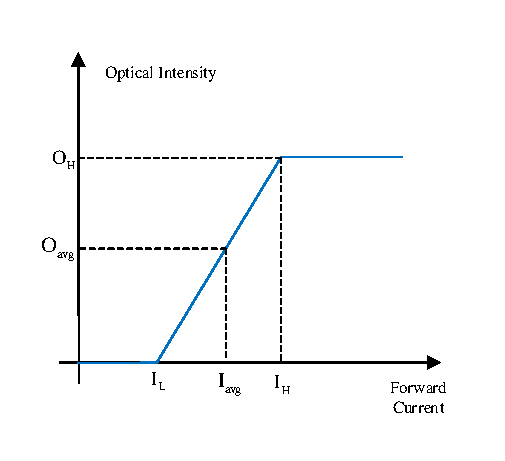
\includegraphics[width=\linewidth]{figures/LED_IO.pdf}
  \caption{Linearized LED I-O characteristic.}
  \label{fig:LEDIO}
\end{figure}

\begin{equation}
  R_x(t)= \gamma T_x(t) \otimes h(t) + n(t),
  \label{eq:channelResponse}
\end{equation}
where $R_x(t)$ denotes received electrical signal, $\gamma$ is photodiode responsivity, $T_x(t)$ 
represents forward electrical signal at the transmitter, $h(t)$ is the impulse response of VLC channel, 
$n(t)$ is additive white Gaussian noise (AWGN), and $\otimes$ is an operator of convolution. 

\subsection{Peak-to-Average-Power Ratio}

Literature \cite{tellado2006multicarrier} presents the definition of PAPR 
of multicarrier signals as

\begin{equation}
  PAPR=10\log_{10}{\frac{\max\limits_{0 \leq n < N}{{|x_n|}^2}}{E\{{|x_n|}^2\}}} (dB),
  \label{eq:PAPR}
\end{equation}
where $x_n$ represents modulated signals and $E\{\cdot\}$ denotes the expectation of random variables.

Different from conventional OFDM signals, subsymbols $\mathbf{X}$ carried by subcarriers must be restrict to conjugate 
symmetry in order to generate real time-domain signal. The time-domain signal sample $x_n$ on the $n_{th}$ subcarrier is equivalent to

\begin{equation}
  x_n = \frac{2}{\sqrt{N}} \sum\limits_{k=1}^{N/2-1} |X_k| \cos{\left[\frac{2 \pi kn}{N}+\arg (X_k)\right]},
\end{equation}
where $N$ denotes the number of OFDM subcarriers, $X_k$ is the subsymbol on the $k$th subcarrier, and operator $\arg( \cdot )$ obtains the argument.

In applications, data tends to be random prior to modulation, and sample of subsymbols $X_k \left(k \in \{1,2,\ldots,\frac{N}{2}-1\}\right)$ 
can be approximated as independent discrete uniform random variables. As each sample $x_n$ is a linear combination of independent and identically distributed (i.i.d) random variables, its 
limiting distribution asymptotically approached the Gaussian distribution with zero mean and variance $E\{{|x_n|}^2\}=\sigma_x^2$ when $N$ is so large that the Central Limit Theorem applies.
The power of signal samples is denoted as $p_x=x_n^2$, whose probability density function (PDF) can be described as 

\begin{equation}
  f_{p_x}\left(p\right) = \left\{ \begin{array}{ll}
    \frac{1}{\sqrt{2\pi}\sigma_x} p^{-1/2} e^{-p/2\sigma_x^2}, & p > 0 \\
    0, & p \leq 0. 
  \end{array} \right.
\end{equation}

Then, the cumulative distribution fucntion (CDF) is written as 

\begin{equation}
  F_{p_x}(\gamma)=\int\limits_{0}^{\gamma} \frac{1}{\sqrt{2\pi}\sigma_x} p^{-1/2} e^{-p/2\sigma_p^2}  dp = \frac{2}{\sqrt{\pi}} \int\limits_{0}^{\sqrt{\frac{\gamma}{2\sigma_x^2}}} e^{-p^2} dp.
\end{equation}

Under the assumption that samples in one OFDM symbol are mutally uncorrelated, the CDF of the random variable $PAPR\{x\}$ is lower bounded by 

\begin{align}
  Prob\{PAPR\{x_n\}<\gamma\} & \geq prob{\left\{\frac{{|x_i|}^2}{E\{{x_n}^2\}}<\gamma, i=0,1,\ldots,N-1 \right\}} \\
  & = {\left(Prob\left\{\frac{{|x_n|}^2}{E\{{|x_n|}^2\}}<\gamma\right\}\right)}^N \\
  & = {\left[F_{p_x}\left(\gamma\right)\right]}^N, 
\end{align}
where $Prob\{\cdot\}$ represents the probability of an event.
Then, the CCDF is lower bounded by 

\begin{equation}
  Prob\{PAPR\{x_n\} \geq \gamma\} \leq 1-{\left[F_{p_x}\left(\gamma\right)\right]}^N.
\end{equation}

\section{Tone Reservation in VLC}

Literature \cite{tellado2006multicarrier} proposed a PAPR reduction method based on the TR in real-time OFDM system. Analogous to \cite{yu2015low}, the problem of PAPR minimization for the DCO-OFDM system could 
be recast as a linear program and it can be rewritten as

\begin{align}
  & \max\limits_{\bar{\mathbf{C}}} \quad \mathbf{t} \\
  & \textrm{s.t.} \quad
  \left( \begin{array}{cc}
    \mathbf{Q} & -\mathbf{1}_N \\
    -\mathbf{Q} & -\mathbf{1}_N
  \end{array} \right)
  \left( \begin{array}{c}
    \bar{\mathbf{C}} \\
    \mathbf{t}
  \end{array} \right)
  \leq
  \left( \begin{array}{c}
    -\mathbf{y} \\
    \mathbf{y}
  \end{array} \right),
  \label{eq:optimization}
\end{align}
where $\bar{\mathbf{C}}$ is composed to PAPR reduction signals and $y$ represents original time-domain signals with reserved subcarriers of zero-value.

Meanwhile reserved tones for PAPR reduction with varying position schemes perform differently.
In VLC OFDM systems, generally there exist some subcarriers with SNRs too low to bear information, hence these subcarriers must go 
unused and are available for PAPR reduction. In practical applications, filter is always used and subcarriers in high frequencies 
have quite low SNRs. Considering the low-pass property of VLC system, the reserved tones for PAPR reduction can be allocated on the high-
frequency subcarriers whose SNRs are too low to be useful.

Let ${\left\{M_k\right\}}_{k=0}^{N/2-R/2-1}$ be a sequence of 
source data, which are generated firstly. Then, we insert zero on the positions of peak reduction subcarriers and map the data onto OFDM subcarriers $\left\{Y_k\right\}$ 
with Hermitian symmetry, $\left\{Y_k\right\}$ expressed as,

\begin{figure}[t]
  \centering
  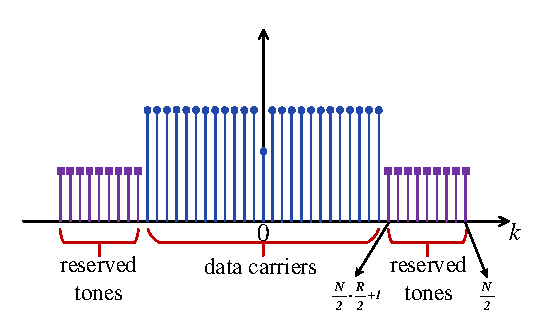
\includegraphics[width=\linewidth]{figures/Subcarriers.pdf}
  \caption{Subcarrier assignment for the proposed TR-based VLC-OFDM}
  \label{fig:subcarriers}
\end{figure}

\begin{equation}
  Y_k = \left\{ \begin{array}{ll}
    0, & k=0 \\
    M_k, & k \in {\left(\mathbb{R}/2\right)}^C \\
    0, & k=N/2, \\
    M_{N-k}^*, & k \in {\left(\mathbb{R}/2\right)}^C
  \end{array} \right.
\end{equation}
where $\mathbb{R}/2=\left\{N/2-R/2+1,\ldots,N/2\right\}$ and ${\left(\mathbb{R}/2\right)}^C$ denotes the complement of $\mathbb{R}/2$ in $\mathbb{N}/2$ and 
$\mathbb{N}/2=\left\{0,1,\ldots,N/2\right\}$. We present the subcarriers assignment for the TR-based 
VLC-OFDM signals in figure \ref{fig:subcarriers}, where the subset of reserved tones $\mathbb{R}$ is deployed onto the reserved tones 
and the data subset $\mathbb{R}_C$ is assigned onto the data subcarriers. Formed as the equation (\ref{eq:optimization}), the optimization expression can help 
to calculate reduced signals $c(t)$, then $c(t)$ is added to $y(t)$ and combined as PAPR reduced OFDM signals $\bar{y}(t)$.


\section{Optimization of Tone Reservation Rate}

As we observed, there exists an optimal tone reservation rate (TRR) that maximizes ergodic communication rate ($Rate$) under various noise scenarios, which would be explained elaborately later. 
Here, we present an adaptive algorithm to adjust TRR to VLC channels under various noise scenarios.

The forward current signal $z(t)$ drives the LED which in turn converts the amplitude of input electrical signal $z(t)$ into optical intensity. The forward signal $z(t)$ is generated 
from the PAPR reduced OFDM signal $\bar{y}(t)$ via both a linear scaling and biasing operation such that

\begin{equation}
  z(t)=\alpha \bar{y}(t) + B,
\end{equation}
where $\alpha$ denotes scaling factor, and $B$ denotes bias sigal.

In order to ensure $z(t)$ within the dynamic range of LED, we can obtain that $\alpha$ should satisfy

\begin{equation}
  \alpha = \max\{\alpha^{(+)}, \alpha^{(-)}\},
\end{equation}
where $\alpha^{(+)}$ and $\alpha^{(-)}$ are respectively defined as

\begin{align}
  \alpha^{(+)} & = \min \left\{\frac{I_H-B}{\max\limits_{t \in (0,T])}{\bar{y}(t)}}, \frac{I_L-B}{\min\limits_{t \in (0,T])}{\bar{y}(t)}}\right\} \\
  \alpha^{(-)} & = \max \left\{\frac{I_H-B}{\min\limits_{t \in (0,T])}{\bar{y}(t)}}, \frac{I_L-B}{\max\limits_{t \in (0,T])}{\bar{y}(t)}}\right\}.
\end{align}

Supposing that $B$ is fixed to $(I_L+I_H)/2$, the dynamic range $D=I_H-I_L$ is also fixed, which is determined by the characteristics of LED. Then, the variance 
of $z(t)$ can be given by

\begin{align}
  \sigma_z^2 & = \alpha^2 \sigma^2_{\bar{y}} \\
  & = \frac{D^2}{4} \frac{\sigma^2_{\bar{y}}}{\max\limits_{t \in (0,T]}{\bar{y}^2(t)}}.
\end{align}

We observe that the scaling factor $\alpha$ is determined by the peak signal of $\bar{y}(t)$ with the fact that a high 
value of peak signal results in inefficient power gain.

Define the dynamic-range-to-noise power ratio (DNR) as $DNR \triangleq G^2D^2/\sigma_n^2$, where $G$ indicates the channel gain with pre-equalization of the channel 
and $\sigma_n^2$ denotes the variance of additive Gaussian noise induced by the receiver.
Combining with the TR approach, define TRR as $TRR \triangleq R/N$, we obtain the SNR for each DCO-OFDM symbol as

\begin{align}
  SNR & = \frac{G^2\alpha^2\sigma^2_s}{\sigma^2_n} \\
  & = \frac{G^2D^2\sigma_s^2}{4\cdot \sigma_n^2 \max\limits_{t \in (0,T]} {\bar{y}^2(t)}} \\
  & = \frac{DNR}{4} \frac{\sigma_s^2}{\max\limits_{t \in (0,T]}{\bar{y}^2(t)}},
\end{align}
where $\sigma_s^2$ denotes signal power carried by the data subcarriers and calling $\sigma_c^2$ as the power of PAPR reduced signal carried by the reserved tones. 
As we known, the signal power of $\bar{y}(t)$ is equivalent to $\sigma^2_{\bar{y}}=\sigma^2_s (1-TRR) + \sigma^2_c TRR$ and the power of original OFDM signal $x(t)$ 
is written as $\sigma_x^2=\sigma_s^2 (1-TRR)$. According to the definition of PAPR with regard to the combined signal $\bar{y}(t)$, SNR can be reformulated as

\begin{equation}
  SNR = \frac{DNR}{4 PAPR_{\bar{y}}} \frac{1}{1-TRR}
  \label{eq:SNR_TRR_},
\end{equation}
where $PAPR_{\bar{y}}$ is represented as the PAPR of the additive signal $\bar{y}(t)$, expressed as

\begin{equation}
  PAPR_{\bar{y}} = \frac{\max{\bar{y}(t)}}{\sigma^2_{\bar{y}}}.
\end{equation}

According to the Shannon capacity formula, the ergodic achievable rate, as a function of DNR and TRR, is given by

\begin{figure*}[t]
  \centering
  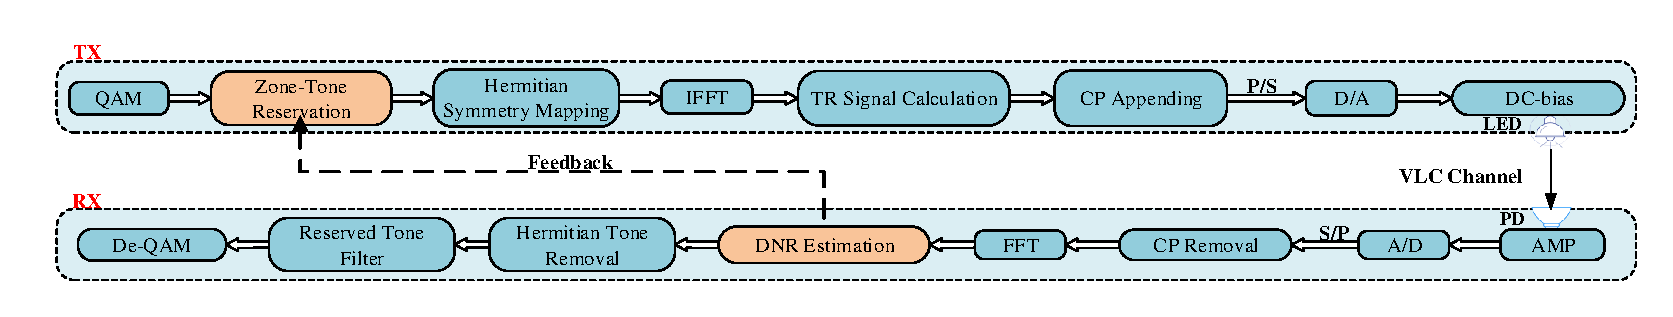
\includegraphics[width=\linewidth]{figures/Ada_DCO_TR_System.pdf}
  \caption{Block diagrams of the propesed TR-based DCO-OFDM VLC system with adaptive TRR algorithm.}
  \label{fig:ada_DCO_TR}
\end{figure*}

\begin{align}
  Rate(DNR,TRR) & = \frac{1-TRR}{2} E_{PAPR_{\bar{y}}}{\left\{\log_2(1+SNR)\right\}} \\
  & = \frac{1-TRR}{2} E_{PAPR_{\bar{y}}}{\left\{\log_2(1+\frac{DNR}{4 PAPR_{\bar{y}}} \frac{1}{1-TRR})\right\}},
\end{align}
As we known, $PAPR_{\bar{y}}$ is decreasing with increasing number of peak reduction tones 
verified by simulations and results. Thus, we can infer that when more subcarriers are available for peak reduction, SNR goes rising 
attribute to the increment of linear scaling and the reduction of noise power on data subcarriers. There exist trade-offs between DNR and TRR. Ensure that TRR falls in a region 
$TRR \in [0,1]$. In term of the equation (\ref{eq:SNR_TRR_}), it can be observed when TRR gets large, SNR increases but ratio of subcarriers carrying with data is declining. 
As a result, there exists trade-off between TRR and data rates. Given the DNR and position of reserved tones 
for peak reduction, we can obtain the optimal $TRR^*$ that maximizes the ergodic achievable data rates as 

\begin{equation}
  TRR^* = \mathop{\arg\max}_{TRR} R|_{DNR}.
  \label{eq:opt_TRR}
\end{equation}

We propose an adaptive TRR scheme based on real-time SNR in VLC. As noise power is estimated periodically and subsequently DNR is evaluated, the optimal TRR can be calculated with equation (\ref{eq:opt_TRR}). 
With this novel scheme, DCO-OFDM VLC system can achieve the maximum data rate using TR technology.

\section{Adaptive TRR Selection Algorithm}

In this section, the proposed adaptive algorithm is illustrated in detail to adjust TRR to VLC channels with various noise scenarios. DNR-TRR lookup tables (LUTs) can be obtained off-line for DCO-OFDM symbols 
with various baseband modulations and are supposed to be stored in memory chips. Once DNRs are estimated initially, the corresponding optimal $TRR^*$ will be calculated using the LUTs. 
Subsequently, signals for peak reduction will be evaluated and mapped onto the positions of reserved tones.

Summarily, the operation steps of the proposed adaptive TRR selection scheme are listed in algorithm \ref{alg:ATS} and the DCO-OFDM system based on adaptive tones adjustment is 
depicted in figure \ref{fig:ada_DCO_TR}.

\begin{breakablealgorithm}
  \caption{The Adaptive TRR Selection Algorithm}
  \label{alg:ATS}
  \begin{algorithmic}[1]
  \Require ~~
  Number of subcarriers, $N$; 
  LUTs of the optimal TRRs, $LUT$;
  \Ensure ~~
  The optical transmitting singal, $T_x$;
  \State Estimating noise power periodically via training symbols by using the Maximum-Likelihood estimator or other estimators for noise power, $\sigma^2_\mathcal{N}$;
  \State Calculating $DNR$ with $\sigma^2_\mathcal{N}$ at receiver;
  \State Constructing receiver Channel State Information (CSI) and sending back to transmitter.
  \State Checking in $LUT$ and obtain the corresponding $TRR^*$ with the estimated $DNR$ at transmitter;
  \State Determing number $Num$ and positions $Idx$ of the reserved tones in accordance with the acquired $TRR^*$;
  \State Constructing transmitter CSI and propagating to receiver;
  \State Calculating the peak reduction signals $C_x$ and mapping the signals $C_x$ onto $Idx$ at transmitter;
  \State Combining with messages subcarriers $M_x$ and generating complete OFDM signals $\bar{y}$;
  \State Converting to analog electrical signals by DACs and subsequently performing linear scaling and DC-bias operation, $\bar{Y}$; 
  \State Modulating the light intensity with the forward electrical signals and transmit the optical signals, $T_x$;
  \State \textbf{return} $T_x$;
  \end{algorithmic}
  \end{breakablealgorithm}

The scheme in this section takes only $O(1)$ complexity but consumes certain amount of storage and calculation for LUTs off-line. The scheme we proposed performs well in practical 
examinations we conduct in next section.

\section{Experimental Setup and Discussion}

In this section, the availability and efficiency of our proposed TR PAPR reduction in VLC OFDM system is demonstrated, and ergodic achievable data rates of the schemes are evaluated and 
compared under varying TRRs and channel noise scenarios. Experimental setup is displayed in figure \ref{fig:experiment}. At the transmitter, signals generated in PC are normalized 
and imported to an arbitrary waveform generator (AWG) designed by field programing gate array (FPGA) and data-analog converter (DAC), 
superimposed on a direct current (DC) bias tee, amplified by high-power amplifier (HPA) and then exploited to drive LED to transmit the signals through light channel. At the receiver, a len is used to concentrate light signals on photodiode 
(PD) converter having 0.5 $mm^2$ active-area and 3dB bandwidth of 350 MHz which transforms light signals to electrical signals. The received signals are shown at a real-time 
oscilloscope (OSC) and recorded by FPGA after analog-data converter (ADC). Most of signal processings such as OFDM digital signal generation are performed off-line by Matlab (PC Software). The devices and instruments all are 
specified in table \ref{tab:dev}.

\begin{figure}[tb]
  \centering
  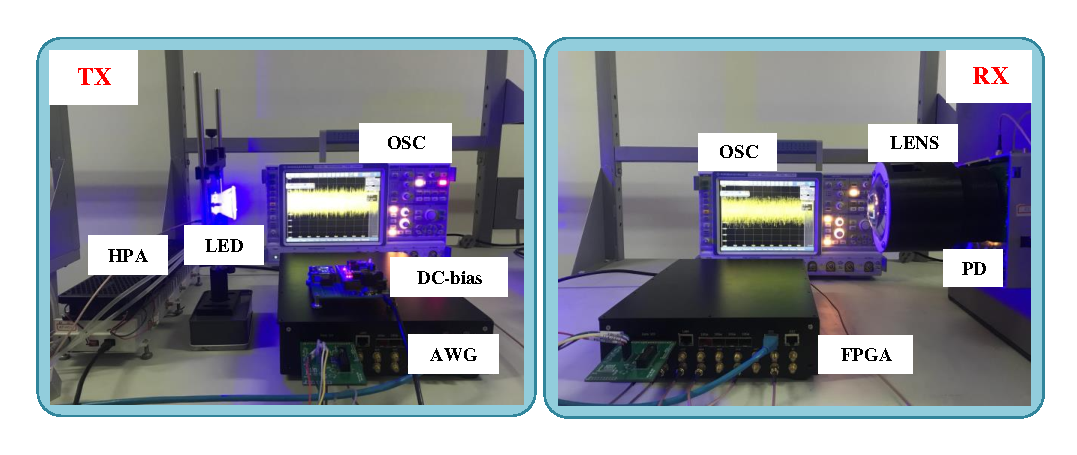
\includegraphics[width=\linewidth]{figures/Experiment.pdf}
  \caption{Experimental setup of our VLC testbed.}
  \label{fig:experiment}
\end{figure}

As metioned above, channel response $h(t)$ in VLC is measured and fitted 
experimentally. In our experimental measures, 
setting light distances between transmitter and receiver as 0.5m, 1m, 2m, Figure \ref{fig:channel} depicts 
spectrum of VLC channel. The $3dB$ bandwidth of the LED channel achieves $15MHz$ due to the limited modulation bandwidth of LEDs.

\begin{figure}[tb]
  \centering
  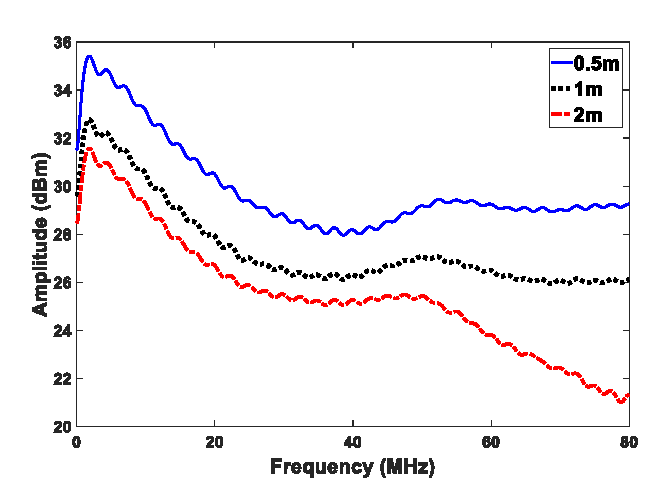
\includegraphics[width=\linewidth]{figures/ChannelSpec.pdf}
  \caption{Measured frequency response of the VLC channel.}
  \label{fig:channel}
  \end{figure}

In the OFDM subcarriers, we set the number of total subcarriers $N_{FFT}=256$ and the sampling speed of DAC and ADC is $f_s=160MHz$ such that the bandwidth of system including message subcarriers and reserved tones 
is shown as $B=80MHz$ due to Hermitian symmetry. In this work, 16QAM is used to modulate binary messages in overall message subcarriers. Besides, considering that the channel in VLC system has a low-pass effect, adaptive QAM 
modulation is also adopted for effectively utilization of channel, which means high order modulation signals are assigned onto the low frequency subcarriers and low order modulation is used in the high frequency subcarriers. 
In the adaptive QAM modulation, 64QAM, 16QAM and 4QAM are employed in different tones respectively. As the high frequencies tones are chosen for PAPR reduction, numbers of reserved tones can be calculated as 
$TRR \times \frac{N_{FFT}}{2}$. The total transmission length of the sequence is 10000 OFDM symbols. 

Setting the rate of reserved tones as $TRR=0, 10\%, 30\%$, respectively, figure \ref{fig:CCDF} compares CCDF curves of PAPR of adaptive QAM modulation format with 16QAM format based on proposed TR 
technique. These curves represent the probability that the PAPR of a DMT block is greater than some value and the results below show that the proposed reserved tones assignment scheme can significantly reduce the PAPR and 
larger TRR can obtain lower PAPR statistically. Comparing to 16QAM modulation, adaptive QAM modulation has excessive PAPR attribute to their higher average power.

The solid lines in figure \ref{fig:PeakPower} fitted for discrete measured points shows the relation between peak value decrease and tone reservation rate, where blue line represents the adaptive QAM modulation format and red 
line denotes 16QAM modulation. Furthermore, the two solid lines imply that the peak value cuts off with TRR increasing and a reduction of almost $35$ percent of peak value in two modulations can be observed if 
enough tones are utilized for PAPR reduction. It is shown that the peak value of the transmitting signals can be decreased when the proposed TR technique is adopted. In our experiment, signals are normalized prior to AWG, which means the peak 
value of transmitting signals could be limited to a constant. In practice, we obtain the amplify of origin signals due to the PAPR reduction, which causes that the effective power of received signals is boosted. The effective 
power denotes the power of signals removing the PAPR reduced signals. The dashed fitted curves in figure \ref{fig:PeakPower} shows the relationship between increasing ratio of effective power and tone reservation rate concerning adaptive QAM 
modulation and 16QAM modulation. There are almost $10dB$ increment of effective power when TRR reachs out $90\%$. Besides, we observe that the two modulations behave similar in increasing of effective power.


\begin{figure}[t]
  \centering
  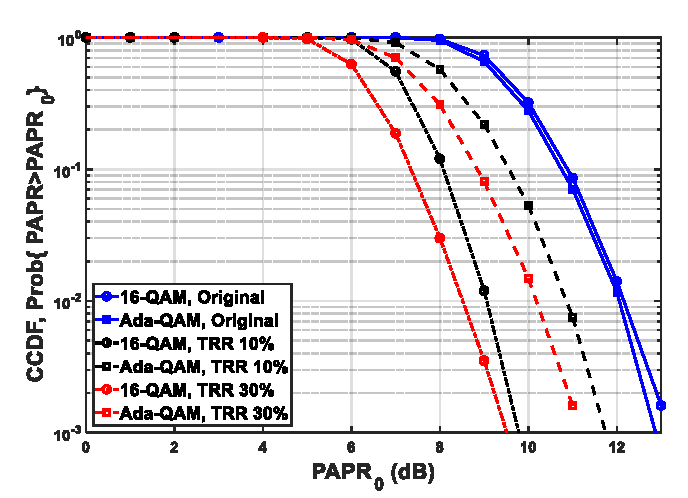
\includegraphics[width=\linewidth]{figures/CCDF.pdf}
  \caption{CCDF of DCO-OFDM based on proposed TR technique in VLC system.}
  \label{fig:CCDF}
\end{figure}

\begin{figure}[t]
  \centering
  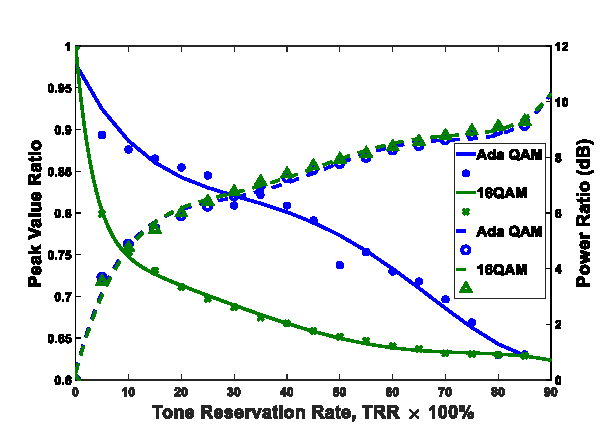
\includegraphics[width=\linewidth]{figures/PeakPower.pdf}
  \caption{Peak value decrease ratio and signal power increase with regard to TRRs in VLC system.}
  \label{fig:PeakPower}
\end{figure}

Figure \ref{fig:R0} and figure \ref{fig:R50} exhibit waveforms and spectrums of AWG output signals we captures from oscilloscope, where original signals without reserved tones are shown in figure \ref{fig:R0} and signals with the proposed TR technique ($TRR=50\%$) 
are shown in figure \ref{fig:R50}. In this work, adaptive QAM modulation scheme is adopted such that ladder-like shape can be found in spectrums of output signals. Otherwise, compared with the waveform of original signals, the counterpart of signals with the proposed 
TR technique performs more steady, which refers to lower PAPR and more effective power ratio. Attribute to occupation of PAPR reduction signals in high-frequency band, high-frequency of spectrum in figure \ref{fig:R50} (40MHz\~80MHz) has higher power than high-frequency 
of spectrum in figure \ref{fig:R0}.

\begin{figure}[t]
  \centering
  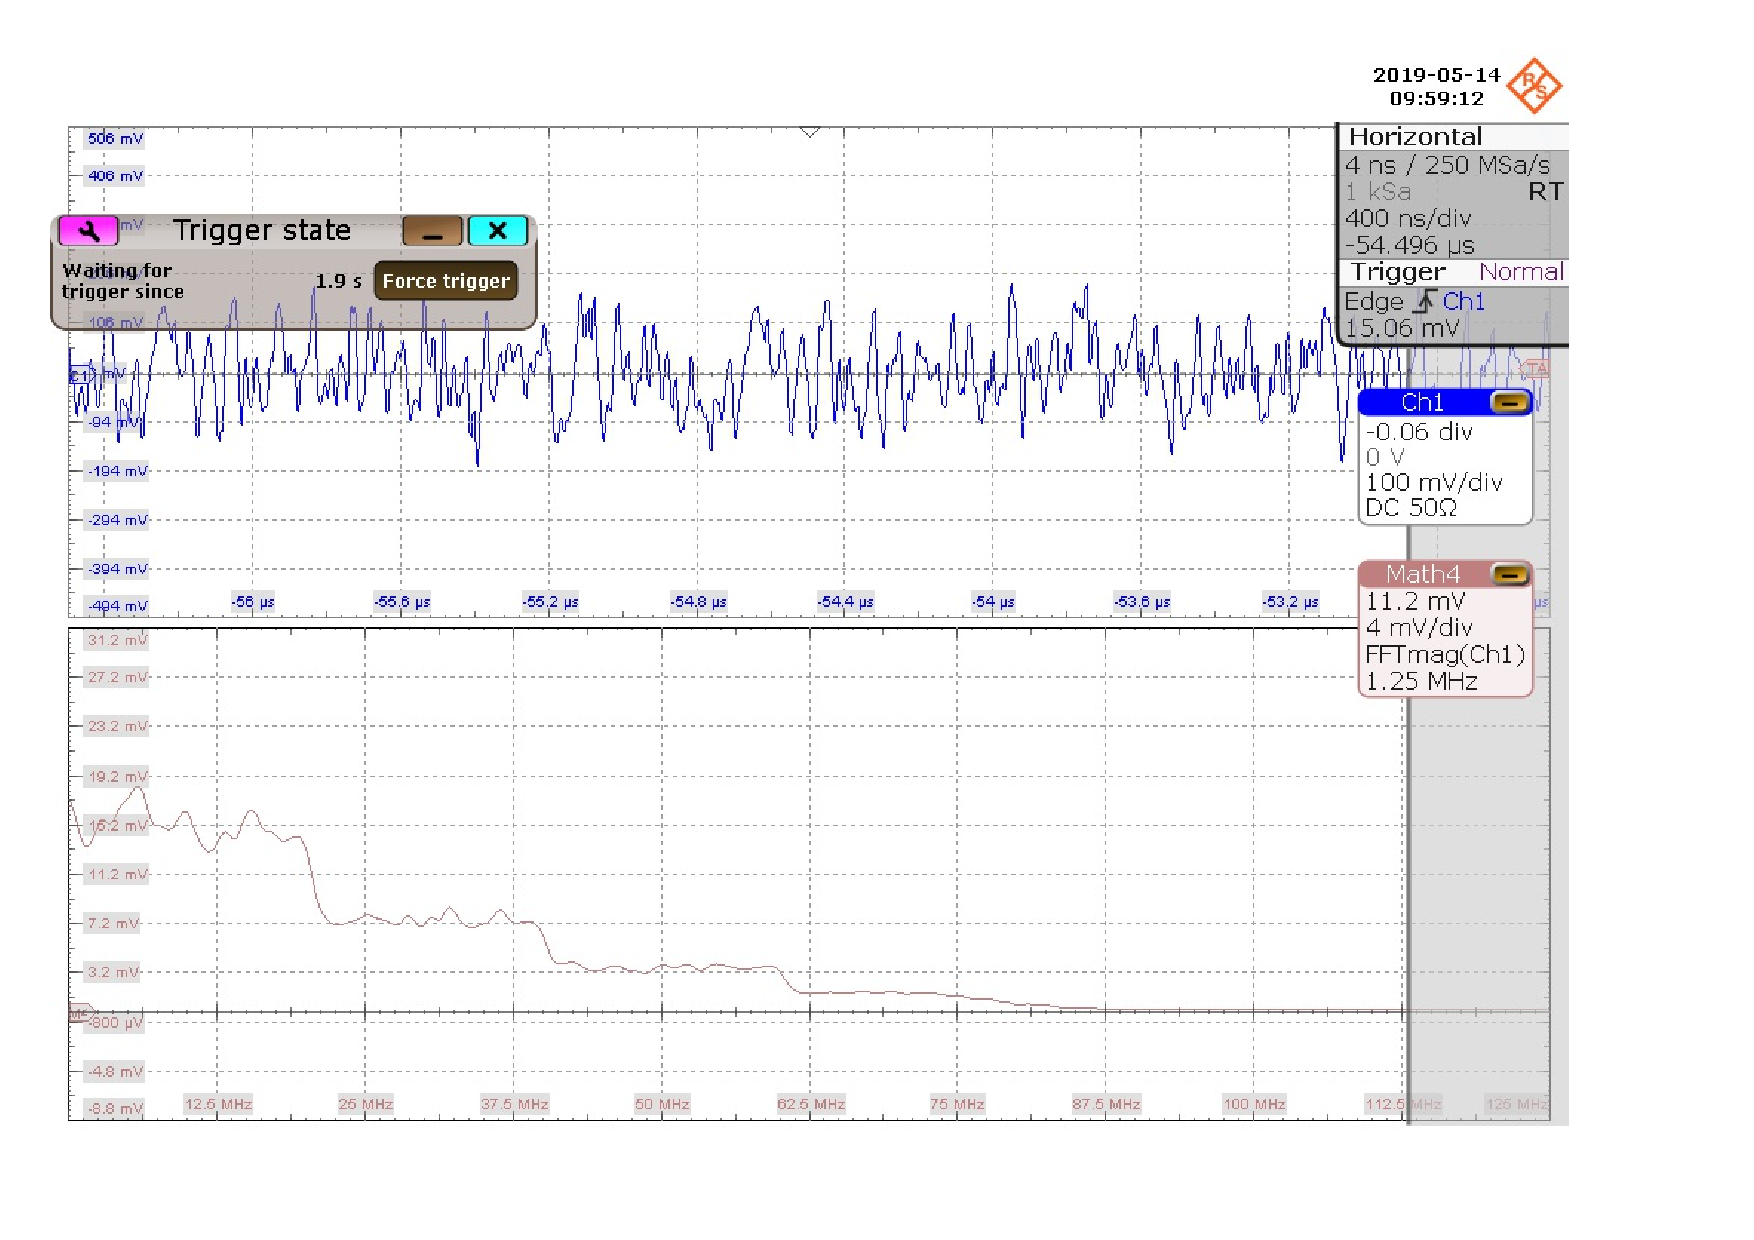
\includegraphics[width=\linewidth]{figures/250M_R0.pdf}
  \caption{Waveform (top) and spectrum (down) of AWG output signals without tone reservation.}
  \label{fig:R0}
\end{figure}

\begin{figure}[t]
  \centering
  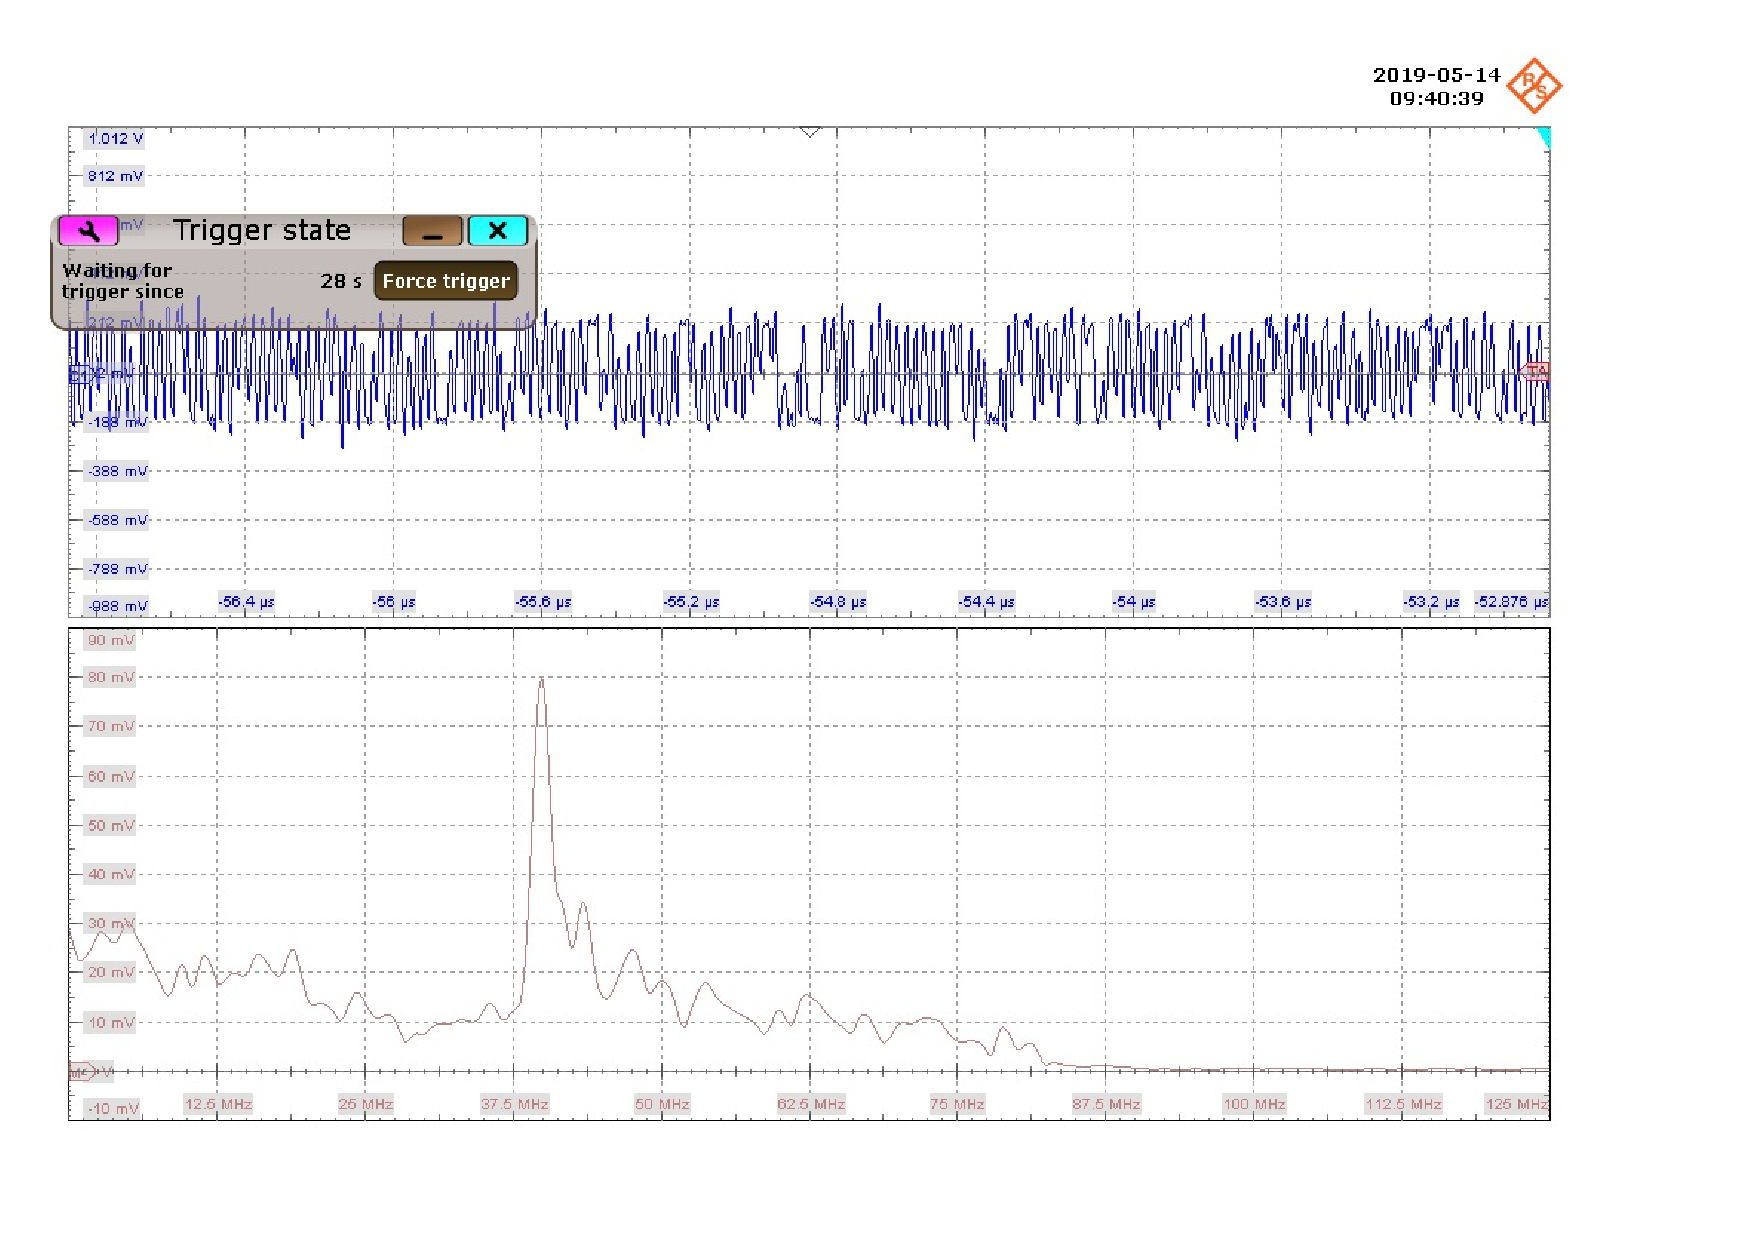
\includegraphics[width=\linewidth]{figures/250M_R50.pdf}
  \caption{Waveform (top) and spectrum (down) of AWG output signals with tone reservation ($TRR=50\%$).}
  \label{fig:R50}
\end{figure}

Figure \ref{fig:TRR_R} demonstrates the relationship between TRR and ergodic achievable rate in QAM-DCO-OFDM systems in varing scenarios of DNRs. Generally, there exists an optimum $TRR^*$ which maximizes the ergodic achievable data rate under a certain DNR scenario.

On the basis of the proposed algorithm \ref{alg:ATS}, we can obtain the optimal TRRs corresponding to DNRs varing from $-5dB$ up to $30dB$ and display the relations between optimal TRR with DNR in 
figure \ref{fig:DNR_TRR}. To be specific, we have measured the relations of DNR and TRR by employing 
adaptive QAM modulation and 16QAM modulation respectively, where DNRs are sampled from $-5dB$ up to $30dB$ uniformly, and subsequently the smoothed curves are evaluated with Gaussian fitting. As shown 
in figure \ref{fig:DNR_TRR} the dash line represents for the result with adaptive QAM modulation 
and the solid line represents 16QAM modulation. Furthermore, we download and analyze the received 16QAM signals with the case of $8dB$ of DNR and the received adaptive QAM signals with the case of $13dB$ 
of DNR, individually. In the cases, the received 16QAM signals have suitable reserved tones with $TRR=50\%$ and the 
received adaptive QAM signals have optimal reserved tones with $TRR=30\%$. The spectrums of the received signals can be evaluated off-line and shown in figure \ref{fig:DNR_TRR}. After synchronization, FFT 
demodulation and equalization, the constellations could be acquired and displayed in figure \ref{fig:DNR_TRR}.

\begin{figure}[]
  \centering
  \subfigure[]{
    \begin{minipage}[t]{0.45\linewidth}
      \centering
      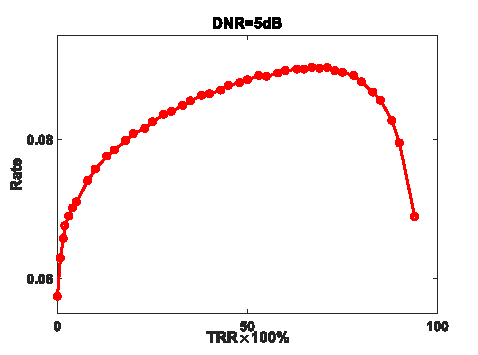
\includegraphics[width=\linewidth]{figures/TRR_R_DNR_5.pdf}
    \end{minipage}
  }
  \subfigure[]{
    \begin{minipage}[t]{0.45\linewidth}
      \centering
      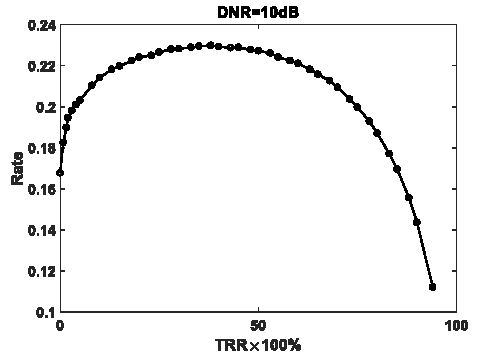
\includegraphics[width=\linewidth]{figures/TRR_R_DNR_10.pdf}
    \end{minipage}
  }
  \caption{(a) The relations between TRR and the achievable ergodic rate in the cases of DNR=5dB. (b) The relations between TRR and the achievable ergodic rate in the cases of DNR=10dB.}
  \label{fig:TRR_R}
\end{figure}

\begin{figure}[t]
  \centering
  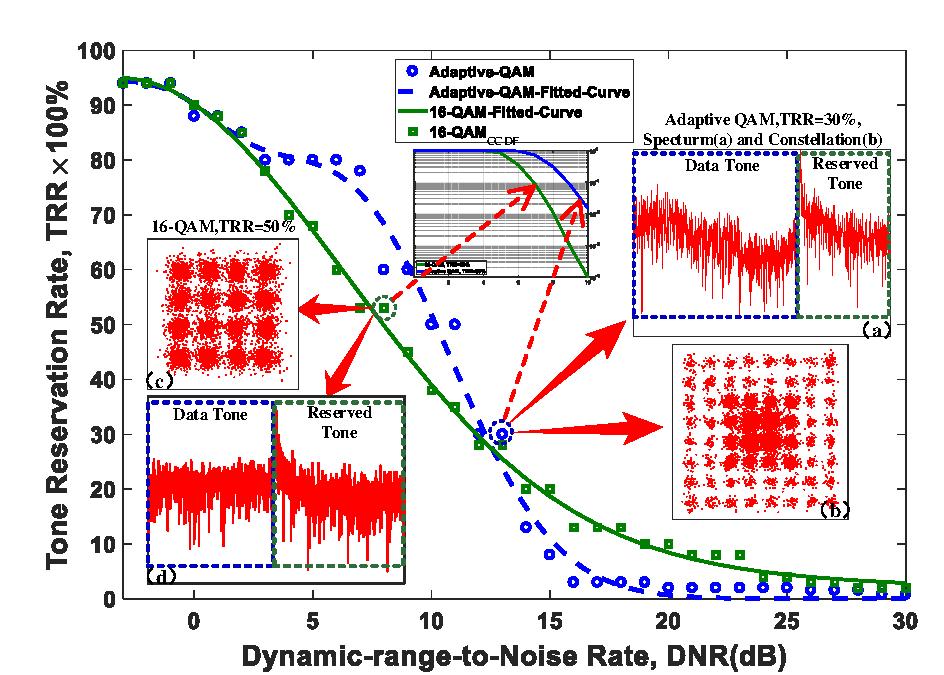
\includegraphics[width=\linewidth]{figures/DNR_TRR.pdf}
  \caption{The relationships between optimal TRRs and DNR concerning 16QAM scheme and adaptive QAM scheme. (a)The spectrum of received adaptive QAM signals in $DNR=13dB$. (b)The constellation of 
  received adaptive QAM signals in $DNR=13dB$. 
  (c)The spectrum of receiver 16QAM signals in $DNR=8dB$. (d)The constellation of 16QAM signals in $DNR=8dB$.}
  \label{fig:DNR_TRR}
\end{figure}

\begin{table}[htb]
  \caption{Instruments and Specifications}
  \begin{tabular*}{8cm}{lll}
  \hline
  Instruments & Specifications \\
  \hline
  FPGA & Xilinx, Virtex-7 \\
  DAC & TI, DAC37j84 \\
  DC bias tee & Mini-Circuits, ZFBT-6GW+ \\
  HPA & Mini-Circuits, ZHL-3A+ \\
  LED & LUMILED, L1C1 \\
  Len & Edmund Optics, \#37-824. \\
  PD & First Sensor, AD800-11 \\
  OSC & Rohde\&Schwarz, RTE1000 \\
  ADC & ADI, AD9680 \\
  \hline
  \end{tabular*}
  \label{tab:dev}
\end{table}

\section{Conclusion}

We design and experimentally demonstrate an novel reserved tone selection scheme for the TR-based DCO-OFDM VLC system. Attributed to the fact that there is certain amount of high frequency band with SNRs 
too low for transmitting messages, those subcarriers in high frequencies can be selected as reserved tones 
for peak reduction. With the proposed TR technique, a significant PAPR reduction is achieved for the DCO-OFDM VLC system. Approximate 35\% reduction of peak-to-peak amplitude is achieved. which 
remarkably relaxed the linear requirement of the electrical transmitter, such as LEDs. Under the constraint 
of the fixed dynamic range of LEDs, almost $10dB$ effective power increment can be achieved by employing the TR technique, which can enhance the performance of VLC system at low SNRs. 
For the purpose of maximizing ergodic achievable rate, an adative TRR scheme is proposed for tradeoff 
between the proportion of data subcarriers and SNR of signals. The proposed scheme performs well in practice and out experiment proves its validness.

\section{Funding Information}

The work  was supported in part by the National Key R\&D Program of China under Grant 2018YFB2202200, in part by the National Natural Science Foundation of China under Grant 61571118.


% \section{References}

% Bibliography
\addcontentsline{toc}{section}{reference}
\nocite{1}
\nocite{*}
\bibliography{MyReference}




% Please include bios and photos of all authors for aop articles
\ifthenelse{\equal{\journalref}{aop}}{%
\section*{Author Biographies}
\begingroup
\setlength\intextsep{0pt}
\begin{minipage}[t][6.3cm][t]{1.0\textwidth} % Adjust height [6.3cm] as required for separation of bio photos.
  \begin{wrapfigure}{L}{0.25\textwidth}
    
\includegraphics[width=0.25\textwidth]{john_smith.eps}
  \end{wrapfigure}
  \noindent
  {\bfseries John Smith} received his BSc (Mathematics) in 2000 from The University of Maryland. His research interests include lasers and optics.
\end{minipage}
\begin{minipage}{1.0\textwidth}
  \begin{wrapfigure}{L}{0.25\textwidth}
    
\includegraphics[width=0.25\textwidth]{alice_smith.eps}
  \end{wrapfigure}
  \noindent
  {\bfseries Alice Smith} also received her BSc (Mathematics) in 2000 from The University of Maryland. Her research interests also include lasers and optics.
\end{minipage}
\endgroup
}{}


\end{document}
